\documentclass[11pt]{article}
\usepackage[english]{babel}
\usepackage[utf8]{inputenc}
\usepackage{hyperref}
\usepackage{fancybox,graphicx}
\usepackage{subfig}
\usepackage{fancyhdr}
\usepackage[left=3.7cm,top=4cm,right=3.7cm,bottom=4cm]{geometry} 
\usepackage{url}
\usepackage{textcomp}
\usepackage{array}
\usepackage{enumitem}
\usepackage{caption}

\hypersetup{
	plainpages = false, pdfpagelabels,
	bookmarks,
	bookmarksopen = true,
	bookmarksnumbered = true,
	linktocpage,
	% pagebackref,
	colorlinks = true,
	linkcolor = blue,
	urlcolor  = blue,
	citecolor = green,
	anchorcolor = green,
	hyperindex = true,
	hyperfigures,
	pdfauthor={Francisco Javier Pérez Gil},
	pdfcreator={Francisco Javier Pérez Gil},
	pdftitle={Trabajo de Interacción y Visualización de la Información: Tableau}
}

\DeclareFontFamily{\encodingdefault}{\ttdefault}{\hyphenchar\font=`\-}
\graphicspath{{./img/}}

\lhead{}
\chead{\textsc{Scife User Guide}}
\rhead{}
\lfoot{Fco. Javier Pérez Gil \& Raúl Moreno Galdón}
\cfoot{}
\rfoot{\thepage}

\renewcommand{\headrulewidth}{0.5pt} 
\renewcommand{\footrulewidth}{0.4pt} 
\pagestyle{fancy}

\renewcommand{\labelitemi}{$\bullet$}
\renewcommand{\labelitemii}{$\circ$}
\renewcommand{\labelitemiii}{$\triangleright$}

\setlength{\parindent}{0pt}
\begin{document}
\thispagestyle{empty}
\begin{titlepage}
	\begin{center}
		\textsc{\Huge ScifE User Guide}
		\vspace*{0.5in}\\
		\huge{\textsc{Universidad de Castilla-La Mancha}}
		\vspace*{0.6in}\\
		\begin{figure}[h!]
			\centering
			\subfloat{
				
\includegraphics[scale=0.40]{logo_esii}}
			\hspace{.5cm}
			\subfloat{
				
\includegraphics[scale=0.60]{uclm.jpg}}
		\end{figure}
		\vspace{0.6in}
		\huge{\textbf{Authors:}\\Francisco Javier Pérez Gil\\Raúl Moreno Galdón}
	\end{center}
\end{titlepage}
\newpage
\thispagestyle{empty}
\tableofcontents
\clearpage
\thispagestyle{empty}
\listoffigures
\clearpage
\setcounter{page}{1}

\section{Introduction}
This document contains a user manual that explains the user how to use the ScifE application. Information is structured in different sections, each one contains the instructions of a subject: experiment, applications, and so one.

\section{Experiments}
This section explains the user how to operate with the experiment functionality offered in the ScifE application.

\subsection{Index}
The main view of experiment is the index. The user can access this view clicking the ``Experiments'' URL in the navbar (see Figure \ref{fig:index} in yellow colour). As you can see, the index view (Figure \ref{fig:index}) shows a experiment list with a brief info of each experiment. All the experiment are showed in an accordion, clicking the name of an experiment you can deploy its information. The colour bar of each experiment change its colour, depending of the experiment status. For example, in the Figure \ref{fig:index}, the \texttt{X CESM} has a green colour bar, this is because its status is done. But for example, the \texttt{BCN CESM} show its bar in red colour, because its status has some error.\\
\begin{figure}[htp]
	\centering
	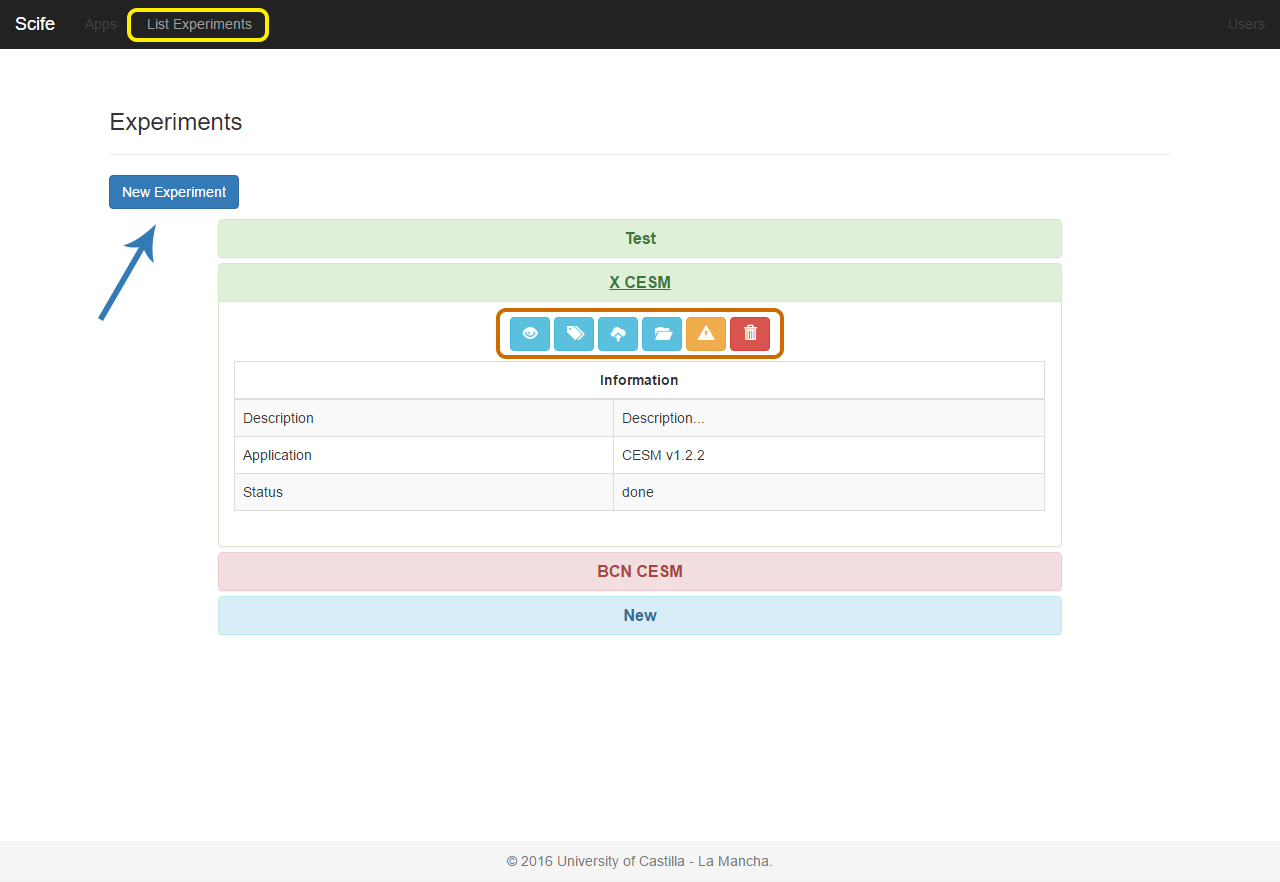
\includegraphics[width=\linewidth]{index}
	\caption{Experiment index view.}
	\label{fig:index}
\end{figure}

When you deploy an experiment, you will see some info and buttons. For example, the Figure \ref{fig:index} shows the ``X CESM'' experiment deployed with the next information:
\begin{itemize}
	\item Description: in this field the user will see the the info inserted when the experiment was created.
	\item Application: this field shows the name of the application associated with the experiment. In this case ``CESM v.1.2.2''
	\item Status: finally, the user can see the status of the experiment, besides of the colour bar.
\end{itemize}

You can also see a series of buttons in each experiment (see Figure \ref{fig:index} marked in orange colour). This buttons allow the user browse the application functions of the experiment in question:
%todo Completar cada boton con la referencia a cada sección
\begin{itemize}
	\item The first button (eye open) redirect the user to the overview view, learn more in Section \ref{sec:overview}.
	\item The second button redirects the user to the labels view, see in Section \ref{sec:labels}.
	\item The next button opens a new view that allows the user upload files to experiment, see more in Section \ref{sec:inputData}.
	\item The button with a open folder redirects the user to sources view, see in Section \ref{sec:sources}.
	\item The yellow button redirects the user to the logs view (Section \ref{sec:logs}).
	\item Finally, the red button with a trash allows the user delete an experiment. When you click this button, a modal view appear to confirm the user action as you can se in the Figure \ref{fig:index-delete}. 
\end{itemize}

\begin{figure}[htp]
\centering
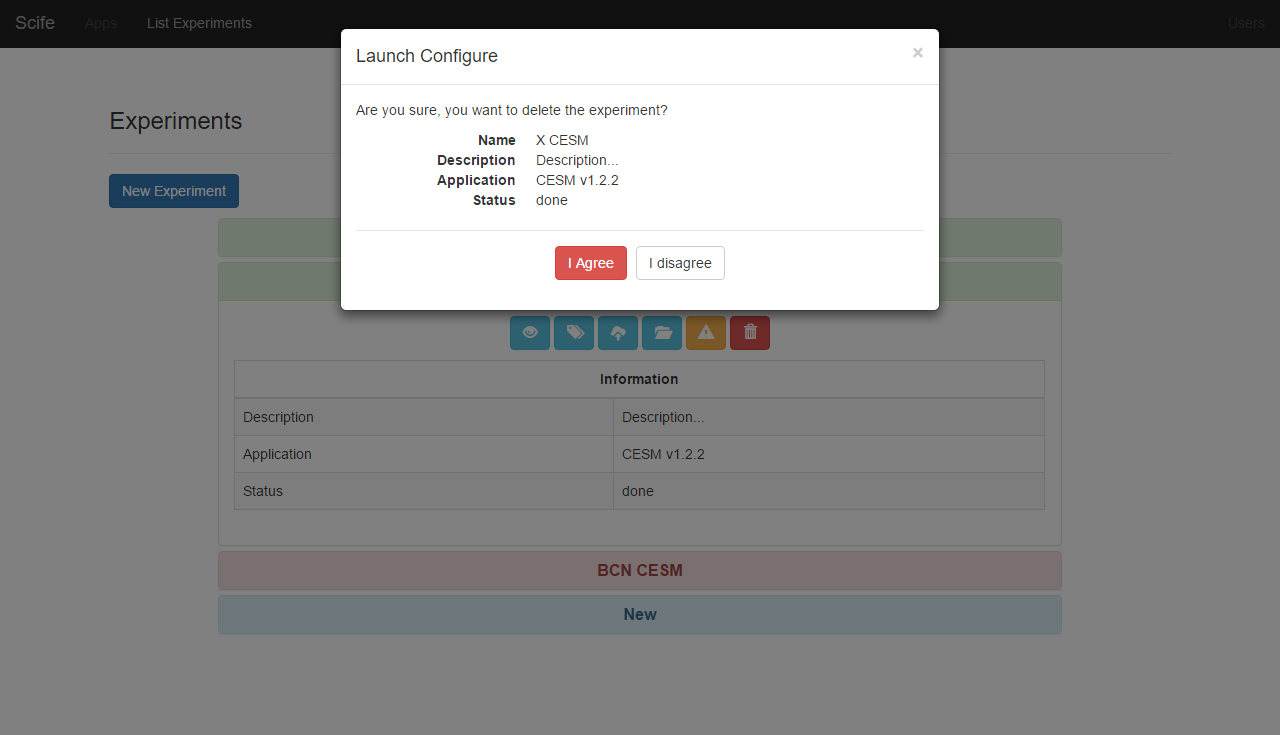
\includegraphics[width=\linewidth]{img/index-delete}
\caption{Modal view to confirm the deletion experiment.}
\label{fig:index-delete}
\end{figure}

From the index view, you can create new experiments, only have to click the ``\texttt{New Experiment}'' button. After that, a new view will appear, like the showed in the Figure \ref{fig:create}. You need input some information to create the new experiment like its name, description or the application in which the experiment will be executed.
\begin{figure}[htp]
	\centering
	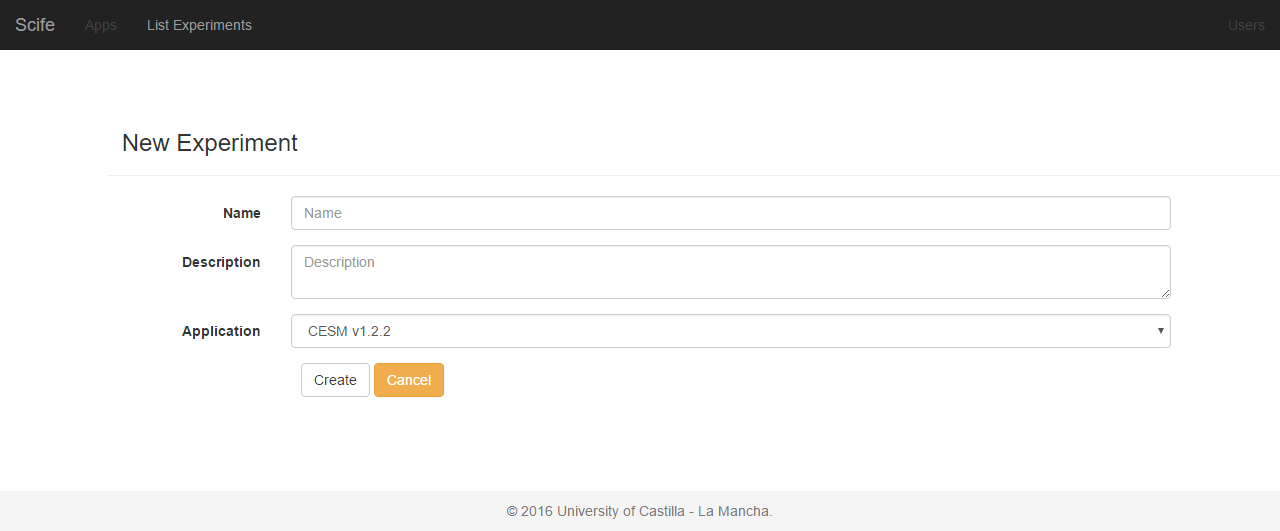
\includegraphics[width=\linewidth]{img/create}
	\caption{View with the form to create a new experiment.}
	\label{fig:create}
\end{figure}

\subsection{Overview}\label{sec:overview}
The overview is the main view of an experiment, in this page you can launch, reset, delete the experiment or download the results when the execution has finished. See the Figure \ref{fig:overview-done} as example, notice the buttons in the centre of the page:
\begin{figure}[htp]
	\centering
	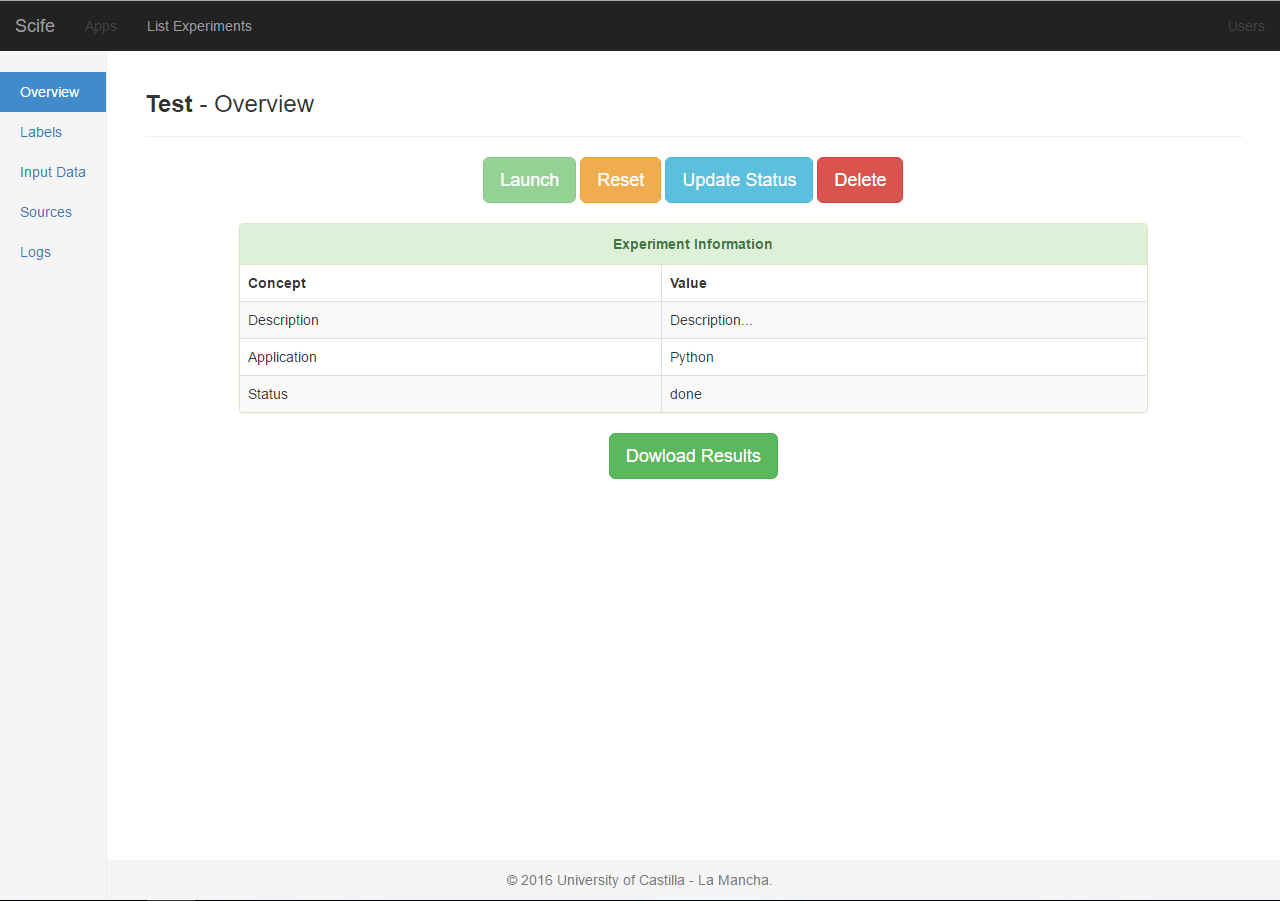
\includegraphics[width=\linewidth]{img/overview-done}
	\caption{The overview view.}
	\label{fig:overview-done}
\end{figure}

\begin{itemize}
	\item Launch button, allow the user execute the experiment. This button only is available when the experiment status is ``created''. When you click this button, the launch modal view will appear, as you can se in the Figura \ref{fig:overview-launch}. In the launch modal you must select the number of nodes, the image and the size of each node where the experiment will be executed. Besides, in the bottom of the modal, you will see information about the cluster where you will execute the experiment, ``Fedora Science'' in this case.
	\item The reset button allows the user stop the experiment execution.
	\item With the ``Update Status'' you can refresh the experiment status to known its status (launched, failed, done, etc.).
	\item Finally, the ``Delete'' button allows delete the experiment. Before do that, appear a modal view to confirm the deletion as you can see in the Figura \ref{fig:overview-delete}.
\end{itemize}

\begin{figure}[htp]
	\centering
	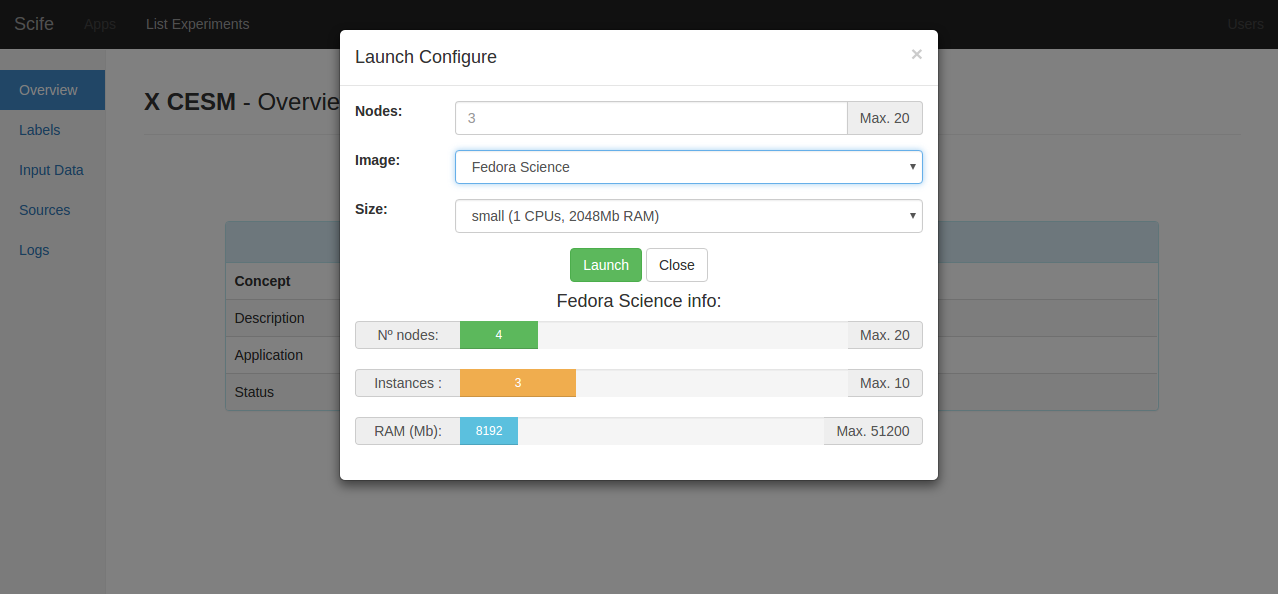
\includegraphics[width=\linewidth]{img/overview-launch}
	\caption{The launch modal view in the overview page.}
	\label{fig:overview-launch}
\end{figure}
\begin{figure}[htp]
	\centering
	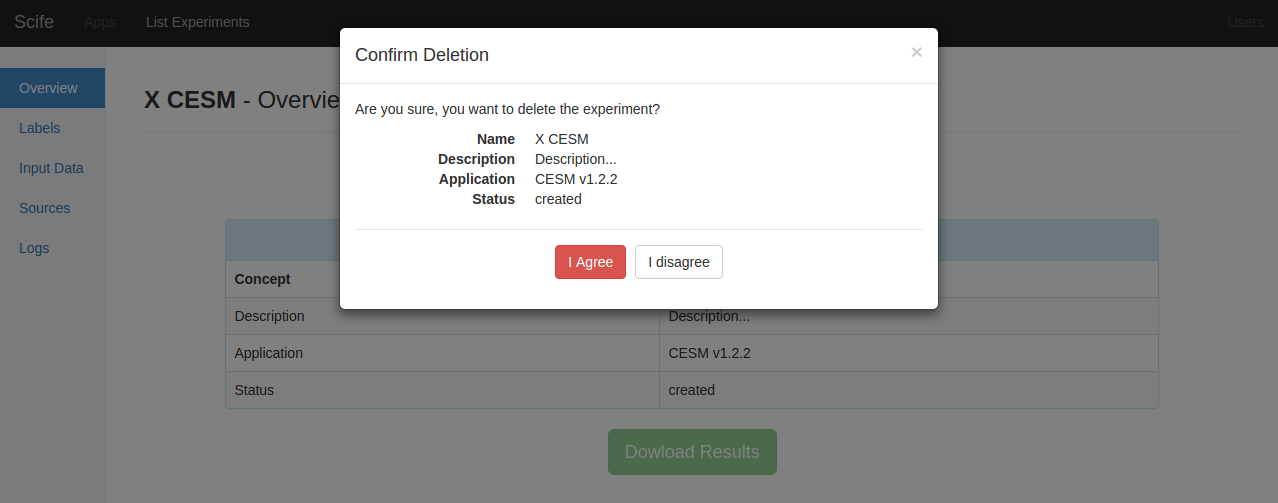
\includegraphics[width=\linewidth]{img/overview-delete}
	\caption{Confirm deletion modal view in the overview page.}
	\label{fig:overview-delete}
\end{figure}
\subsection{Labels}\label{sec:labels}
\subsection{Input data}\label{sec:inputData}
\subsection{Sources}\label{sec:sources}
\subsection{Logs}\label{sec:logs}

\end{document}
